\subsection{Current Solution}
\label{description:solution}
Currently, Tomboy has the functionality to create bullet lists in notes and with help of the backlink addin (which is shipped with the default Tomboy installation) to add links between different notes. This allows the user to create simple task lists through bullet lists and through linking a single task to another note to create subtasks. This functionality is also shown in the GUI Mock-up in Figure \ref{gui}.

In the past, there have been several official and unofficial attempts to come up with an addin for handling tasks in Tomboy which however all did not result in a satisfactory end product due to missing functionality or integration. Our goal is to implement such a project up to a stable and working solution, such that it could eventually be included in the Tomboy project and shipped with future Tomboy releases. 

Since those earlier projects directly influenced some of our design decisions with respect to \textit{bug-rareness}, \textit{usability} and \textit{integration into Tomboy}, section \ref{appendix:history} goes into detail about some of those projects and why they failed to achieve their requirements.

\subsection{Product Perspective}
\label{description:perspective}
  The project \textit{TaskManager For Tomboy} will be part of the Tomboy project.\\
  Figure \ref{perspective} shows the Product perspective of the TaskManager addin. Since it's really an extension for Tomboy it is placed in
  the addins section of Tomboy itself where it will communicate with some of Tomboys internal elements (as shown by connecting lines).
  \begin{itemize}
    \item TaskManager will directly customize the Tomboy Note Writer user interface in a way that the user can write task lists in notes 
	(this functionality can be seen in Figure \ref{gui}. To achieve this TaskManager will  directly rely on some of the 
	widgets in the GTK\# library. The corresponding requirements for this are documented in section \ref{requirements:interfaces:user}.
    \item Opening an existing note should also load the defined task lists with tasks and display them automatically in the note - in other words:
    tasks have to be made persistent.
	We  will save the task information by using the storage facilities available by Tomboy and extend
    the currently used XML \index{XML} format to store notes. This functionality is covered in section \ref{requirements:interfaces:software:persistence}.
    \item Finally, TaskManager will give the user a way find notes with open tasks or tasks that are overdue. This means we have to modify
    the existing Note Browser user interface. This functionality is covered in requirement \textit{Filter notes} in section \ref{requirements:interfaces:user:filter}.
  \end{itemize}


  \begin{figure}[ht]
    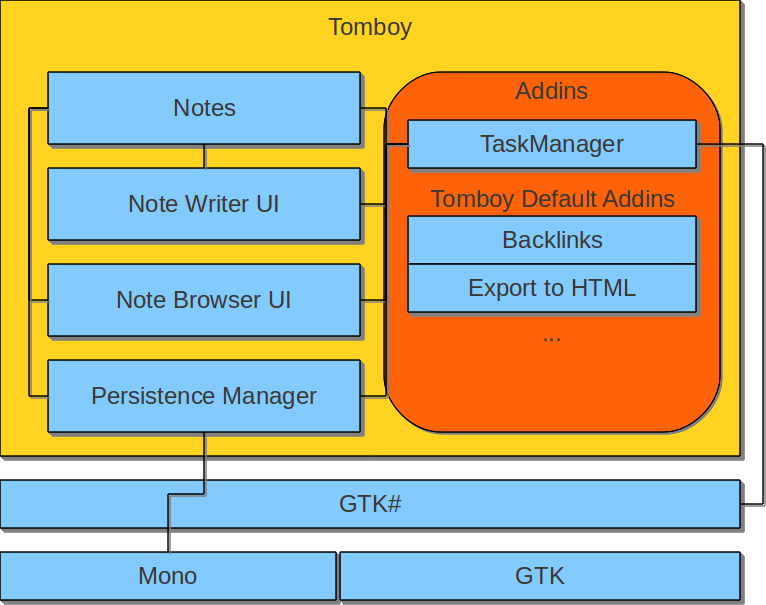
\includegraphics[width=\textwidth]{graphics/product_perspective_diagram.png}
    \caption{TaskManager Product Perspective}
    \label{perspective}
  \end{figure}


\subsection{Product Functions}
\label{description:functions}

  \subsubsection*{Supported Functions}
  \label{description:functions:supported}

    \begin{itemize}
      \item Provides advanced task management capabilities for Tomboy.
      \item Allows multiple tasks to be grouped together.
      \item Supports priorities and due dates for tasks and task lists.
      \item Allows to establish relationships/dependencies between tasks.
      \item Allows the user to conveniently get to the task notes currently not finished or overdue.
      \item Allows to export all defined tasks.
    \end{itemize}

    \subsubsection*{Unsupported Functions}
      \label{description:functions:unsupported}
      \begin{itemize}
        \item Does not introduce additional GUI window elements or external tools within or outside of Tomboy (see \ref{lessons} for the reasoning).
        \item Does not support on-the-fly synchronization with external tools or clients except for manual export.
        \item Does not support importing tasks from other task manager tools.
      \end{itemize}

\subsection{User Characteristics}
\label{description:usercharacteristics}
We look at two types of users:

  \begin{itemize}
    \item[\bf{Casual}] The casual user will create simple task lists. He may not know the various functions of Tomboy very well. Still, he will be able to create simple task lists where he can cross out individual elements easily. \index{Casual User}

    \item[\bf{Advanced}] The advanced user knows and uses Tomboy already quite well. He is able to add arguments such as due dates and priorities to his task lists and tasks, and to create hierarchies of tasks. \index{Advanced User}

  \end{itemize}


\subsection{Constraints}
\label{description:constraints}
The addin itself will obey criteria (standards and guidelines) imposed by the GNOME and Tomboy projects.
Namely these are:
\begin{itemize}
 \item GNOME Human Interface Guidelines
 \item GNOME Documentation Style guide %TODO
 \item GNOME Programming Guidelines
 \item Mono Coding Guidelines
\end{itemize}
The documents can be found by looking at the reference table in section \ref{styleguide}.

Besides the coding guidelines this includes mainly design aspects, such as simplicity and easiness of use, and full integration into Tomboy (see also \ref{lessons}).
